\documentclass[12pt]{article}
\usepackage[spanish]{babel}
\usepackage[utf8]{inputenc}
\usepackage{amsmath}
\usepackage{graphicx}
\usepackage{hyperref}
\usepackage{doi}
\usepackage{mathtools}
\usepackage{float}
\usepackage[colorinlistoftodos]{todonotes}
\usepackage[letterpaper, margin=1.in]{geometry}
\usepackage[version=3]{mhchem}

\begin{document}

\begin{titlepage}

\newcommand{\HRule}{\rule{\linewidth}{0.5mm}}

\center

\textsc{\LARGE Universidad de los Andes}\\[1.5cm]
\textsc{\Large Departamento de F\'isica}\\[0.5cm]
\textsc{\large Biolog\'ia Sint\'etica}\\[0.5cm] 

\HRule \\[0.4cm]
{ \huge \bfseries Proyecto}\\[0.4cm]
\HRule \\[1.5cm]
 

\Large \emph{Autores:}\\
Manuela \textsc{Vanegas Ferro}\\
Juan David \textsc{Estupi\~n\'an M\'endez}\\
Luis Alberto \textsc{Guti\'errez L\'opez}\\[2cm]

\Large \emph{Profesor:}\\
Juan Manuel \textsc{Pedraza Leal}\\[3cm]


{\large Mayo 21 de 2015}\\[2cm]

\vfill

\end{titlepage}

\tableofcontents
\pagebreak

\begin{abstract}
  Your abstract\cite{kressler01} \cite{cleland67} \cite{turlings95} \cite{sallaud09} \cite {kirby09} \cite{harada09a} \cite{harada09b} \cite{crocker80} \cite{engerberg-kulka04} \cite {alon06}.
\todo{aaa}
\end{abstract}

\section{Introducci\'on}


\section{Modelo Matem\'atico}
\label{sec:model}

\begin{figure}[H]
  \centering
  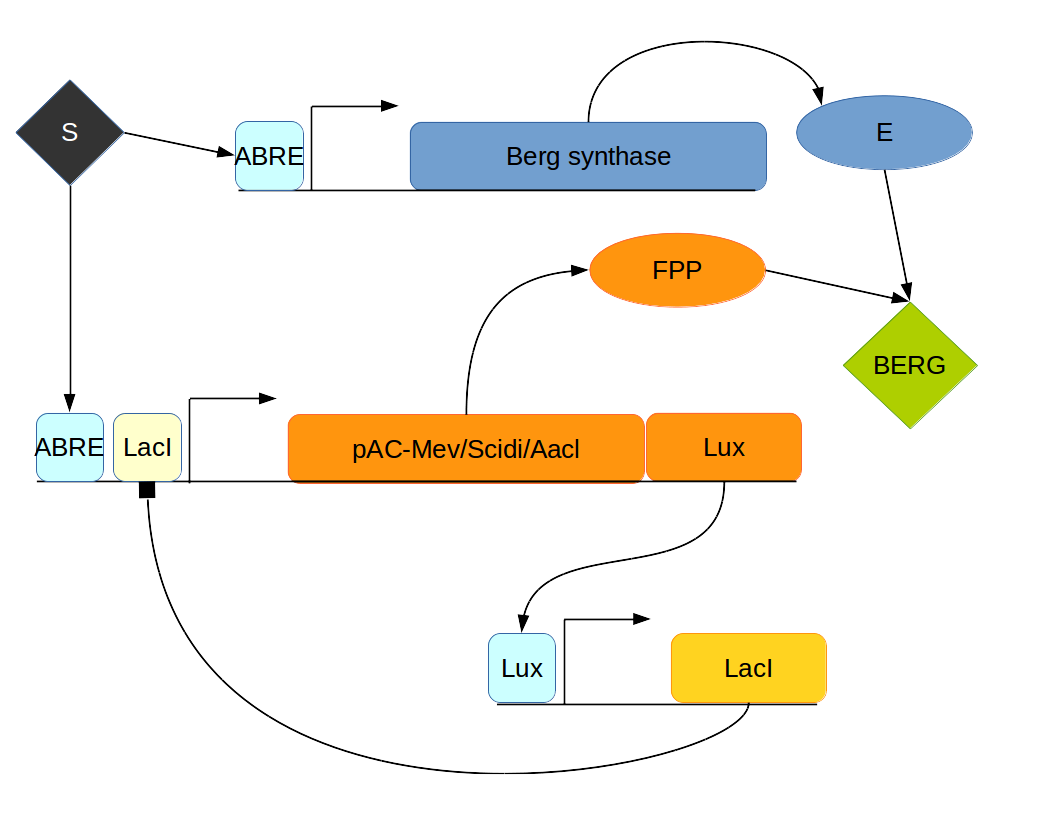
\includegraphics[width=0.5\textwidth]{circuit.png}
  \caption{\label{fig:Circuit}This is a figure caption.}
\end{figure}

\subsection{Ecuaciones de Hill}

Se model\'o la parte transcripcional como se ha hecho en clase y est\'a explicado en \cite{alon06}. Consideramos que el ADN total del gen a transcribir $\text{D}_{\text{T}}$ es constante, es decir:

\begin{equation} \label{eq:D_T}
[\text{D}_{\text{T}}]=[\text{D}]+[\text{DS}]+[\text{DI}]+[\text{DIS}],
\end{equation}

Donde $[\text{D}]$ representa el ADN libre, $[\text{DIS}]$ el ADN unido tanto al represor I como al activador S, $[\text{DS}]$ el unido al activador, y $[\text{DI}]$ el unido al represor.

Para realizar balance detallado se consideraron las siguientes ecuaciones qu\'imicas, las cuales son equivalentes al diagrama del inicio  de la primera tarea del curso.

\begin{align}
\ce{[D] + [S]} &\ce{<=>[\ce{k_{S+}}][\ce{k_{S-}}] [DS]}, \label{eq:rchem1}\\ 
\ce{[D] + [I]} &\ce{<=>[\ce{k_{I+}}][\ce{k_{I-}}] [DI]}, \label{eq:rchem2}\\
\ce{[DS] + [I]} &\ce{ <=>[\ce{k_{I+}}][\ce{k_{I-}}] [DIS]}, \label{eq:rchem3}\\ 
\ce{[DI] + [S]} &\ce{<=>[\ce{k_{S+}}][\ce{k_{S-}}] [DIS]}. \label{eq:rchem4}
\end{align}

Donde las $k$ son las constantes de las respectivas reacciones y se define la constante de disociaci\'on como $K = \frac{k_-}{k_+}$ \cite{alon06}. Seg\'un las ecuaciones qu\'imicas podemos plantear las ecuaciones diferenciales. Al evaluar tiempos mucho mayores a los tiempos en los que ocurre la uni\'on entre el ADN y los factores de transcripci\'on es v\'alido suponer que se ha alcanzado el estado estacionario, obteniendo entonces de las ecuaciones anteriores:

\begin{equation}
\label{eq:Dss}
\dot{[\text{D}]}=0=-k_{S+}[\text{D}][\text{S}]+k_{S-}[\text{DS}]=-k_{I+}[\text{D}][\text{I}]+k_{I-}[\text{DI}],\\
\end{equation}

De donde se tiene que:

\begin{equation}
\label{eq:K1}
[D][S]=K_S[DS], \quad [D][I]=K_I[DI] 
\end{equation}

Ahora se busca hallar la raz\'on entre el ADN en los distintos estados (dados por la ecuaci\'on \ref{eq:D_T}), se realizar\'a detalladamente para $[DS]$. De la ecuaci\'on \ref{eq:K1} se obtiene:

\begin{equation}
\label{eq:DS}
[D] = \frac{K_S}{S}[DS], \quad [DIS] = \frac{I}{K_I}[DS], \quad [DI]=\frac{K_S}{S}[DIS]=\frac{K_S}{S}\frac{I}{K_I}[DS],
\end{equation}

Para incluir los coeficientes de Hill en el modelo, se realiza el mismo an\'alisis pero considerando la posibilidad de que varias mol\'eculas de los factores de transcripci\'on pueden unirse al ADN, siguiendo el procedimiento del ap\'endice A.2 de \cite{alon06} obtenemos un resultado similar a la ec. \ref{eq:DS}, pero con las fracciones dependientes de S e I elevadas a los coeficientes de Hill $n_S$ y $n_I$, respectivamente. Por lo tanto al reemplazar esto en la ec. \ref{eq:D_T} y reorganizando se tiene que:

\begin{equation}
\frac{[DS]}{[D_T]} = \frac{1}{\left( \frac{K_S}{S} \right)^{n_S} + \left( \frac{I}{K_I} \right)^{n_I} \left( \frac{K_S}{S} \right)^{n_S} + 1 + \left( \frac{I}{K_I} \right)^{n_I}},
\end{equation}

La expresi\'on anterior representa la fracci\'on de ADN ligado a $S$ que hay en equilibrio, al considerar un tiempo suficientemente largo para que ocurran muchos eventos de uni\'on y disociaci\'on de los factores de transcripci\'on esto se puede interpretar como la probabilidad de que el ADN se encuentre en este estado y por lo tanto que la transcripci\'on se d\'e en \'el. As\'i, al multiplicar por la fuerza del promotor $\beta$ obtenemos la tasa de transcripci\'on en dicho estado del ADN.

De la misma manera se pueden realizar el an\'alisis para $[DI]$, $[D]$ y $[DIS]$ para obtener las tasas de transcripci\'on en cada uno de los estados. La tasa total es la suma de todas las tasas, donde adem\'as se toma la tasa correspondiente al ADN libre como una constante \todo{Esto por que} $\alpha$. Tambi\'en se sigue un procedimiento similar para hallar la tasa de producci\'on de $r_E$, que es mucho m\'as sencillo pues s\'olo hay un promotor. Se incluye un t\'ermino de degradaci\'on $\gamma$ tanto de ARN como de prote\'inas y se incluye tambi\'en una tasa de creaci\'on de prote\'inas $k_P$ que tomaremos como constante y se determinar\'a seg\'un el RBS.

Las ecuaciones que se obtienen son las siguientes:

\begin{multline}
\label{eq:rZ}
\dot{r_Z}(t) = 
\alpha_{IS}
+ \frac{\beta_{IS_I}}{\left( \frac{K_I}{I} \right)^{n_I} + 1 + \left( \frac{S}{K_S} \right)^{n_S} \left( \frac{K_I}{I} \right)^{n_I} + \left( \frac{S}{K_S} \right)^{n_S}}\\
+ \frac{\beta_{IS_S}}{\left( \frac{K_S}{S} \right)^{n_S} + \left( \frac{I}{K_I} \right)^{n_I} \left( \frac{K_S}{S} \right)^{n_S} + 1 + \left( \frac{I}{K_I} \right)^{n_I}}
+ \frac{\beta_{IS_{IS}}}{\left( \frac{K_I}{I} \right)^{n_I} \left( \frac{K_S}{S} \right)^{n_S} + \left( \frac{K_S}{S} \right)^{n_S} + \left( \frac{K_I}{I} \right)^{n_I} + 1}
- \gamma_{r_Z} r_Z
\end{multline}

\begin{equation}
\label{eq:Z}
\dot{Z}(t) = k_Z r_Z - \gamma_Z Z
\end{equation}

\begin{multline}
\label{eq:rI}
\dot{r_I}(t) = 
\alpha_{IS}
+ \frac{\beta_{IS_I}}{\left( \frac{K_I}{I} \right)^{n_I} + 1 + \left( \frac{S}{K_S} \right)^{n_S} \left( \frac{K_I}{I} \right)^{n_I} + \left( \frac{S}{K_S} \right)^{n_S}}\\
+ \frac{\beta_{IS_S}}{\left( \frac{K_S}{S} \right)^{n_S} + \left( \frac{I}{K_I} \right)^{n_I} \left( \frac{K_S}{S} \right)^{n_S} + 1 + \left( \frac{I}{K_I} \right)^{n_I}}
+ \frac{\beta_{IS_{IS}}}{\left( \frac{K_I}{I} \right)^{n_I} \left( \frac{K_S}{S} \right)^{n_S} + \left( \frac{K_S}{S} \right)^{n_S} + \left( \frac{K_I}{I} \right)^{n_I} + 1}
- \gamma_{r_I} r_I
\end{multline}

\begin{equation}
\label{eq:I}
\dot{I}(t) = k_I r_I - \gamma_I I
\end{equation}

\begin{equation}
\label{eq:r_E}
\dot{r_E}(t) = \alpha_S + \frac{\beta_S}{1+ \left( \frac{K_S}{S}\right)^{n_S}} - \gamma_{r_E} r_E\\
\end{equation}

\begin{equation}
\label{eq:E}
\dot{E}(t) = k_E r_E - \gamma_EE
\end{equation}

\todo[inline]{Mirar si se ponen las condiciones iniciales aqui o que}

\subsection{Reacciones enzim\'aticas}

\todo{explicar mejor, citar una figura por ejemplo} Las reacciones enzim\'aticas en este caso no se pueden modelar directamente utilizando la ecuaci\'on de Michaelis-Menten porque hay dos ecuaciones qu\'imicas para las enzimas y \'estas no son independientes, pues como se ve a continuaci\'on:

\begin{align}
\ce{[Z] + [A]} &\ce{<=>[\ce{\hat{k}_+}][\ce{\hat{k}_-}] [ZA] ->[\ce{\hat{k}_{cat}}] [Z] + [F]}, \label{eq:echem1}\\
\ce{[E] + [F]} &\ce{<=>[\ce{k_+}][\ce{k_-}] [ZA] ->[\ce{k_{cat}}] [Z] + [F]}, \label{eq:echem2}
\end{align}

[F] depende de las dos ecuaciones, incluyendo t\'erminos adicionales en las ecuaciones diferenciales. Las constantes $k$ de las reacciones est\'an dadas y se aproxima la cat\'alisis \todo{?} como una reacci\'on irreversible, lo cual es muy preciso para reacciones enzim\'aticas. Seg\'un lo anterior las ecuaciones diferenciales quedan:

\begin{align}
  \dot{[B]} &= k_{\text{cat}}[E][F]-\gamma_BB \label{eq:Bdot}\\
  \dot{[ZA]} &= \hat{k}_+[Z][A] - \hat{k}_-[ZA]-\hat{k}_{\text{cat}}[ZA] \label{eq:ZAdot}\\
  \dot{[EF]} &= k_+[E][F]-k_-[EF]-k_{\text{cat}}[EF] \label{eq:EFdot}\\
  \dot{[F]} &= -k_+[E][F]+k_-[EF]+\hat{k}_{\text{cat}}[ZA] \label{eq:Fdot}
\end{align}

Como las reacciones enzim\'aticas generalmente ocurren a tasas mucho mayores que los tiempos t\'ipicos de degradaci\'on de las prote\'inas, las tasas de degradaci\'on para los pasos intermedios son despreciables, siendo necesario incluirla \'unicamente en la ecuaci\'on para B. Asumiendo que los complejos enzima-sustrato est\'an en equilibrio \todo{citar?}, es decir, $\dot{[ZA]} = 0$ y $\dot{[EF]} = 0$ obtenemos de las ecuaciones \ref{eq:ZAdot} y \ref{eq:EFdot}:

\begin{align}
[ZA]&=\hat{K}_M[Z][A] \quad \text{donde} \: \hat{K}_M \coloneqq \frac{\hat{k}_+}{\hat{k}_-+\hat{k}_{\text{cat}}},\\
[EF]&=K_{M}[E][F] \quad \text{donde} \: K_M \coloneqq \frac{k_+}{k_-+k_{\text{cat}}},
\end{align}

Donde $K_M$ y $\hat{K}_M$ son las constantes de Michaelis de las reacciones. Reemplazando esto en \ref{eq:Fdot} y reorganizando obtenemos:

\begin{align}
\dot{[F]}&=\hat{k}_{\text{cat}}\hat{K}_M[Z][A]+(k_-K_M-k_+)[E][F], \label{eq:F}\\
\dot{[B]}&=k_{\text{cat}}[E][F]-\gamma_B[B]. \label{eq:B}
\end{align}

Las cuales son las ecuaciones diferenciales para F y B que dependen de las cantidades conocidas, ambas ecuaciones junto con \ref{eq:rZ} - \ref{eq:E} y las condiciones iniciales para cada una de las funciones ser\'an las inclu\'idas en los modelos deterministas y estoc\'astico.

\subsection{Modelo determinista}



\subsection{Modelo estoc\'astico}
Para realizar la simulaci\'on estoc\'astica se utiliz\'o el algoritmo de Gillespie

\bibliographystyle{plain}
\bibliography{written.bib}

\end{document}
